\section{Thermal noise in BJT}

This problem works with the BJT and the objective is to evaluate all three noises: thermal, flicker and shot.

First a simple circuit is assembled with the transistor BFU530 from NXP. Also it is applied two DC voltage sources to polarize the BJT. In this case with $V_{be} = 0.8 V$ and $V_{ce} = 3 V$. An AC simulation is executed from 1 Hz to 10 GHz.

Additionally two DC feeders are added in the connection of each voltage source to its respective BJT node (base and collector). The DC feeder prevent interference between the BJT own noise with another noise source.

First of all we observe in figure \ref{fig:bjt1} the simulation results taking into account all noise sources combined. The first identified noise type is the flicker (or $1/f$ noise), that extends in all frequency range with a decaying characteristic. In $10^5 Hz$ there is a higher decaying rate in the PSD, this marks the end of the constant spot noise and the begin of the cutoff band from the filtering result by the parasite capacitances inherent to the BJT. Last, the thermal noise serves as a background offset the maintains approximately constant all over the frequency range. 

\begin{figure}[H] 
\centering
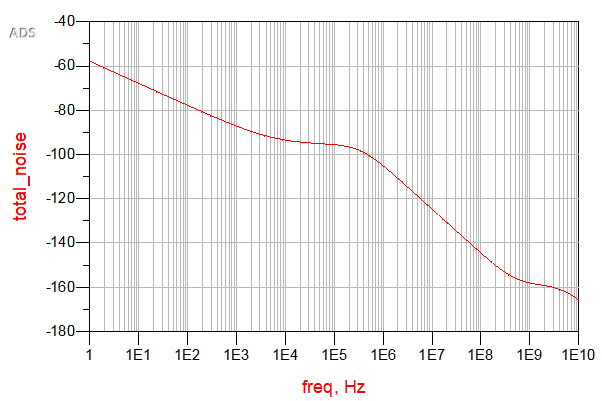
\includegraphics[width=10cm]{images/total_noise.png}
\caption{Noise PSD response for BJT BFU530 from NXP.}
\label{fig:bjt1} 
\end{figure}

A better way to observe each noise source effect is disassembling each component and plotting each contribution separated. The figure \ref{fig:bjt2} show each noise source influence. As mentioned before, the spot noise has a clear white behaviour until the parasite capacitances cutoff at $10^5 Hz$. Different from the spot noise, the thermal noise has a white behaviour that depends only on the temperature and the resistance and keeps constant until approximately $100 THz$. The flicker noise has a $1/f$ behaviour before the cutoff and decays with a higher rate after it.

\begin{figure}[H] 
\centering
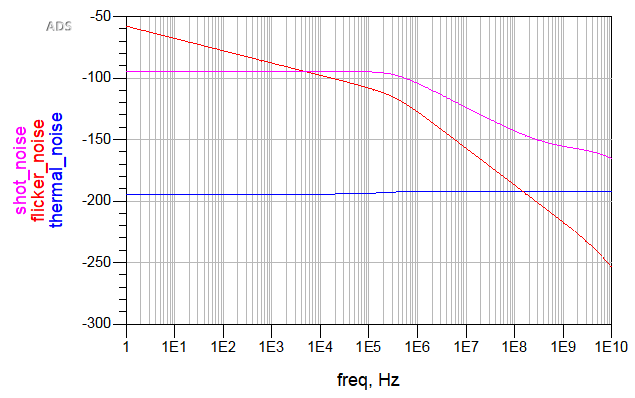
\includegraphics[width=10cm]{images/partial_noise.png}
\caption{Disassembled noise PSD response for BJT BFU530 from NXP.}
\label{fig:bjt2} 
\end{figure}